\documentclass[a4paper,10pt]{article}
\usepackage[utf8]{inputenc}
\usepackage[russian]{babel}
\usepackage{amsmath}
\usepackage{amssymb}

\DeclareMathOperator{\rot}{rot}
\DeclareMathOperator{\mdiv}{div}
\DeclareMathOperator{\RE}{Re}
\renewcommand{\Re}{\mathop{\mathrm{Re}}\nolimits}

%opening
\title{Численное исследование 3-х мерных не изотермических течений несжимаемой жидкости в прямоугольной каверне с подвижной крышкой}
\author{Владимир Олегович Пиманов}
\date{xx.xx.xxxx}

\begin{document}

\maketitle

\begin{abstract}
  aaaaaaa
\end{abstract}

\section{}
  \section*{Введение}

С тех пор, как 

  \section*{Система уравнений Навье-Стокса}


  \section{Математические выкладки}

\subsection{Математическая постановка задачи}

\begin{figure}
  \begin{center}
    \begin{picture}(180,180)(-90,-90)
      \thinlines
      \put(-80,-40){\vector(1,0){160}}
      \put(-40,-80){\vector(0,1){160}}
      %\put(-49,-51){\textsl{0}}
      %\put(37,-51){\textsl{1}}
      %\put(-49,30){\textsl{1}}
      \put(80,-51){\textsl{x}}
      \put(-49,80){\textsl{y}}
      \thicklines
      \put(-40,-40){\line(1,0){80}}
      \put(40,-40){\line(0,1){80}}
      \put(60,40){\line(-1,0){120}}
      \put(60,60){\line(-1,0){120}}
      \put(-40,40){\line(0,-1){80}}
      \put(-60,49.7){\circle{19.5}}
      \put( 60,49.7){\circle{19.5}}
      \put(-10,33){\vector(1,0){30}}
      \put(10,67){\vector(-1,0){30}}
      \thinlines
      \multiput(-40,-40)(0,7){12}{\line(-1,-1){10}}
      \multiput(-40,-40)(7,0){14}{\line(-1,-1){10}}
      \multiput( 40,-44)(0,7){11}{\line(1,1){10}}
      \multiput(-47.5,40)(5,0){20}{\line(0,1){5}}
      \multiput(-47.5,60)(5,0){20}{\line(0,-1){5}}
      \put(53,43){\line(1,1){14}}
      \put(53,57){\line(1,-1){14}}
      \put(-53,43){\line(-1,1){14}}
      \put(-53,57){\line(-1,-1){14}}
    \end{picture}
  \end{center}
  \caption{Каверна с подвижной крышкой}
  \label{pic2D}
\end{figure}

Ставится трехмерная (3D) задача о расчете поля скорости $ \vec v(t) $ в каверне с подвижной крышкой $ \Theta $ . Каверна имеет форму траншеи, бесконечно длинной, с квадратным поперечный сечением $\Theta \times \mathbb{R} \text{, где } \Theta = (0,1) \times (0,1) $. 
Жидкости передается движение крышки $ \Gamma_1 \times \mathbb{R} \text{, где } \Gamma_1 = (0,1) \times {1} $. 
Крышка движется равномерно со скоростью $ \vec{v}_0 = (1,0,0) $. Схематически каверна изображена 
на рисунке \ref{pic2D}. 
Считается, что жидкость вязкая, ньютоновская, несжимаемая, изотермическая, и описывается системой
уравнений Навье-Стокса.
\begin{gather}
  \nabla \cdot \vec v = 0 \label{3D_first}\\
  \frac{\partial \vec v}{\partial t} = \vec v \times \vec \omega - \nabla p - 
  \nu ( \nabla \times \vec \omega ), \text{при } \vec x \in \Theta \times \mathbb{R}\\
  \vec v = (1,0,0), \text{при } \vec x \in \Gamma_1 \times \mathbb{R} \\
  \vec v = (0,0,0), \text{при } \vec x \in \Gamma_2 \times \mathbb{R} \\
  \vec v (0) = \vec v _0 \label{3D_last}
\end{gather}

Здесь $ \vec \omega = \nabla \times \vec v $ - завихренность, p - полное кинематическое давление,
$ \nu = 1 / \Re $ - вязкость, $ \Re $ - число Рейнольдса, $ \Gamma_2 = \partial \Theta \setminus \Gamma_1 $ - боковые стенки и дно каверны, $ \partial \Theta = \Gamma_1 \cup \Gamma_2 $ - 
граница области, $\vec v _0$ - начальное распределение скорости. 

Решение данной задачи \ref{3D_first}\,--\,\ref{3D_last} обозначим как $ \{ \vec V(x,y,z,t), P(x,y,z,t) \} $~--- пара скорость-давление. Тогда $ \{ \vec V(x,y,z), P(x,y,z) \} $~--- стационарное решение этой задачи. 


\subsection{Постановка двумерной задачи}

Хорошо известно, что при достаточно малых числах Рейнольдса в каверне устанавливается двумерное стационарное течение $$ 
  \{\vec V(x,y,z), \vec P(x,y,z) \} = \{[\vec V(x,y), 0], [\vec P(x,y), 0]\}
$$

Здесь $\vec V(x,y)$~--- двумерный вектор скорости, $P(x,y) $~--- давление (скаляр), величины зависят только от двух переменных. Для их нахождения существует двумерная задача, аналогичная задаче \ref{3D_first}\,--\,\ref{3D_last}.
\begin{gather}
  \label{2D_first}
  \nabla \cdot \vec v = 0 \\
  \frac{\partial \vec v}{\partial t} = \vec v \times \vec \omega - \nabla p - 
  \nu ( \nabla \times \vec \omega ), \text{при } \vec x \in \Theta \\
  \vec v = (1,0), \text{при } \vec x \in \Gamma_1\\
  \vec v = (0,0), \text{при } \vec x \in \Gamma_2\\
  \vec v (0) = \vec v _0
  \label{2D_last}
\end{gather}

Здесь вектор $ \vec \omega = \nabla \times \vec v = [0,0,\omega_z]$ имеет компоненту в напралении оси OZ (и только такую компоненту), но в уравнения $ \vec \omega $ входит только в составе выражения $ [(f_x,f_y),0] \times \vec \omega = [(f_y \omega_z, -f_x \omega_z), 0]$, результат которого~--- двумерный вектор, лежащий в плоскости OXY. Систему уравнений \ref{2D_first}\,--\,\ref{2D_last} можно считать двумерной. 

Решение двумерной задачи \ref{2D_first}\,--\,\ref{2D_last} $\{ \vec V, P \}$ далее будет называться \textit{базовым течением}.

\subsection{Линеаризованная система уравнений}

Базовое течение следует проверить на устойчивость к малым трехмерным возмущениям.

Через $\{ \vec v(x,y,z,t), p(x,y,z,t) \} $ обозначены трехмерные \textit{малые возмущения}, наложенные на базовое течение. 
\begin{gather*}
  \vec V(x,y,z,t) = \vec V(x,y) + \vec v(x,y,z,t) \\
  P(x,y,z,t) = P(x,y) + p(x,y,z,t)
\end{gather*}

Новая система уравнений, линейная относительно неизвестных $ \vec v(x,y,z,t)$, $p(x,y,z,t) $, получена путем подстановки выражения в систему уравненй \ref{3D_first}\,--\,\ref{3D_last}. Сокращено принебрежимо малое слагаемое $ \vec v \times \vec \omega $ и использован тот факт, что  $\vec V(x,y), P(x,y) $~--- решение системы \ref{2D_first}\,--\,\ref{2D_last}.
\begin{gather} 
  \label{lin3D_first}
  \nabla \cdot \vec v = 0\\
  \frac{\partial \vec v}{\partial t} = \vec V \times \vec \omega + \vec v \times \vec \Omega - \nabla p - \nu ( \nabla \times \vec \omega ), \text{при } \vec x \in \Theta \times \mathbb{R}\\
  \vec v = (0,0,0), \text{при } \vec x \in \partial \Theta \times \mathbb{R} \\
  \vec v (0) = \vec v _0 \label{lin3D_last}
\end{gather}

Здесь $\vec V = \vec V(x,y) $~--- базовое течение, $ \vec \omega = \nabla \times \vec v $, $ \vec \Omega = \nabla \times \vec V $~--- завихренность малых возмущений и базового течения соответственно, $\vec v_0$~--- распределение малых возмущений в начальный момент времени t=0. 

Над системой уравнений \ref{lin3D_first}\,--\,\ref{lin3D_last} можно выполнить преобразование Фурье по переменной z и перейти от переменной z к волновому числу $\alpha$.

Функции, над которыми было выполнено преобразование Фурье, обозначены соответствующими буквами готического алфавита. Если f(x,y,z)~--- некоторая функция от трех переменных, тогда $ \mathfrak{f}(x,y,\alpha) $~--- соответствующая ей преобразованная функция.
$$
 \mathfrak{f}(x_0,y_0,\alpha) = \int_\mathbb{R} f(x_0,y_0,z) e^{-i\alpha z} dz 
$$

\if 0
Если считать, что $\vec v = (v_x, v_y, v_z)$, $\vec V = (V_x, V_y)$, $\vec \Omega = (0, 0, \Omega_z)$, то в скалярном виде преобразованную систему можно записать так:
\begin{gather} 
  \label{scalar3D_first}
 \frac{\partial \hat v_x}{\partial x} + \frac{\partial \hat v_y}{\partial y} + i\alpha \hat v_z= 0\\
% 
 \frac{\partial \hat v_x}{\partial t} = \vec V \times \vec \omega + \vec v \times \vec \Omega - \nabla p - \nu ( \nabla \times \vec \omega ), \text{при } \vec x \in \Theta \times \mathbb{R}\\
% 
 \frac{\partial \vec v}{\partial t} = \vec V \times \vec \omega + \vec v \times \vec \Omega - \nabla p - \nu ( \nabla \times \vec \omega ), \text{при } \vec x \in \Theta \times \mathbb{R}\\
% 
 \frac{\partial \vec v}{\partial t} = \vec V \times \vec \omega + \vec v \times \vec \Omega - \nabla p - \nu ( \nabla \times \vec \omega ), \text{при } \vec x \in \Theta \times \mathbb{R}\\
% 
 \vec v = (0,0,0), \text{при } \vec x \in \partial \Theta \times \mathbb{R} \\
 \vec v (0) = \vec v _0 
  \label{scalar3D_last}
\end{gather}
\fi

Также введены следующие обозначения для некоторых линейных операторов.
$$
  \nabla_\alpha = (\frac{\partial}{\partial x},\frac{\partial}{\partial y},-\alpha I)\text{,\qquad} 
  \nabla_\alpha^* = (\frac{\partial}{\partial x},\frac{\partial}{\partial y},\alpha I) 
$$

В таких обозначения система уравнений \ref{lin3D_first}\,--\,\ref{lin3D_last}, над которой было выполнено преобразование фурье, имеет вид
\begin{gather} 
  \label{ft3D_first}
  \nabla_\alpha^* \cdot  \mathfrak{\vec v} = 0\\
  \frac{\partial \mathfrak{\vec v}}{\partial t} = \vec V \times \mathfrak{\vec w} + \mathfrak{\vec v} \times \vec \Omega - 
		\nabla_\alpha \mathfrak{p} - \nu ( \nabla \times \mathfrak{\vec w} ), \text{при } \vec x \in \Theta\\
  \vec v = (0,0,0), \text{при } \vec x \in \partial \Theta\\
  \mathfrak{\vec v} (0) = \vec v _0 \label{ft3D_last}
\end{gather}
Здесь $\mathfrak{\vec w} = \nabla_\alpha \mathfrak{\vec v}$ 

\subsection{Решение спектральной задчачи}

Посколько коэффициетны не в системе уравнений \ref{ft3D_first}--\ref{ft3D_last} не зависят от времени, ей можно сопоставить задачу на собственные значения
\begin{gather} 
  \label{s3D_first}
  \nabla_\alpha^* \cdot  \mathfrak{\vec v} = 0\\
  - \lambda \mathfrak{\vec v} = \vec V \times \mathfrak{\vec w} + \mathfrak{\vec v} \times \vec \Omega - 
		\nabla_\alpha \mathfrak{p} - \nu ( \nabla \times \mathfrak{\vec w} ), \text{при } \vec x \in \Theta\\
  \vec v = (0,0,0), \text{при } \vec x \in \partial \Theta\\
  \mathfrak{\vec v} (0) = \vec v _0 \label{s3D_last}
\end{gather}


Спектральная задача \ref{s3D_first}--\ref{s3D_last} зависит от двух параметров. Это число Рейнольдса Re и волновое число $\alpha$. Для каждой пары (Re,$\alpha$) может быть вычислен спектр задачи $\Lambda(\Re,\alpha)$. Декрементом затухания d(Ra,$\alpha$) называтеся наименьшая из действительных частей собственных значений в спектре.
\begin{gather}
 d(\Re,\alpha) = \min_{\lambda \in \Lambda(\Re,\alpha)} \mathfrak{R}(\lambda)
\end{gather}
Здесь $\mathfrak{R}(c)$ обозначает действительную часть числа c. Пусть декременту соответствует множество собственных чисел $\Lambda_d$:
\begin{gather}
 \Lambda_d(\Re,\alpha) = \{ \lambda \in \Lambda(\Re,\alpha) \mid d = \mathfrak{R}(\lambda) \}
\end{gather}
Вообще говоря, множество $\Lambda_d$ включающее только один элемент.
Составим еще одно множество $V_d$ из собственных векторов, соотвтствующих собственным значниям из определенного выше множества. Решение эволюционной задачи можно представить, как линейную комбинацию решений вида 
\begin{gather}
 V_\lambda e^{-\lambda t}
\end{gather}
Здесь $V_\lambda$ - собственный вектор, соответствующий собственному значению $\lambda$. 
По истечении некоторого времени каждым слагаемым, кроме одного, можно будет пренебречь. Останется то слагаемое, собственное значение которого принадлежит множеству $\Lambda_d$. Если d больше нуля, решение устойчиво, если d 
меньше нуля, решение неустойчиво. Если в множестве $\Lambda_d$ всего одно значение $\lambda_d$, то 
решение будет осциллировать с частотой $\frac{\mathfrak{I}(\lambda_d)}{2\pi}$, где 
$\mathfrak{I}(c)$~--- мнимая часть числа c. Значния $d, V_d, \mathfrak{I}(\lambda_d)$ можно найти 
прямым численным интегрированием задачи \ref{lin3D_first}--\ref{lin3D_last}, не решая задачи на собственные значения.



Для каждого $\alpha$ можно вычислить критическое число Рейнольдса, обозначаемое $\Re_{crit}$, как наименьшее число Рейнольдса, при котором задача теряет устойчивость к возмущениям с длиной волны $\alpha$.
\begin{gather}
 \Re_{crit}(\alpha) = inf\{Re>0 \mid d(\Re,\alpha) < 0\}
\end{gather}
Кривую Re$_{crit}(\alpha)$ назовем \textit{кривой нейтральной устойчивости}. Она определена на плоскости $(\Re,\alpha)$ при $\alpha > 0$. Во всех точках, лежащих ниже кривой,~--- задача устойчива к малым возмущениям. 

В реальном мире возмущения развиваются произвольно. Это значит, что в разложении решения по базису из собственных векторов будет присутствовать каждое слагаемое с ненулевым коэффициентом. 
\textit{Глобальное критическое число Рейнольдса} $\Re_{crit}^*$, параметр исследуемой формы каверны, вычисляется как глобальный минимум кривой нейтральной устойчивости. Если при некотором числе Рейнольдса хотя бы при одном значении волнового числа возмущения нарастают, то есть декремент отрицательный, течение неустойчиво к возмущениям. Если $R^+$~--- множество положительных чисел, то
\begin{gather}
 \Re_{crit}^* = \min_{\alpha \in R^+}(\Re_{crit}(\alpha))
\end{gather}



  \section{Численный метод}

\subsection{Аппроксимация трехмерной системы уравнений}

Для аппроксимации как двумерной задачи, так и линеаризованных уравнений применен метод\cite{method}, поэтому здесь представлен способ аппроксимиции трехмерной системы уравнений как более общий случай.

В работе применен конечно--разностный метод, позволяющий найти решение со вторым порядком точности по пространству и с третьим порядком точности по времени. В расчетной области вводится разнесенная неравномерная сетка. Метод применим только в том случае, когда в области можно ввести ортогональную систему координат, в которой область представляет из себя параллелепипед со стенками, параллельными координатным осям. То есть, если $\Omega$~--- расчетная область, то существуют такие отрезки $l_1, l_2, l_3$, что $\Omega = l_1 \times l_2 \times l_3$. 

\begin{figure}[htp]
  \begin{center}
    \begin{picture}(180,180)(-90,-90)
      \thinlines
     \put(-90,10){\vector(0,1){40}}
     \put(-90,10){\vector(1,0){40}}
     \put(-90,10){\vector(-1,-1){20}}
     \put(-97,46){\text{z}}
     \put(-56,3){\text{y}}
     \put(-110,-2){\text{x}}
      \thicklines
     \put(-30,-30){\line(0,1){60}}
     \put(-30,30){\line(1,0){60}}
     \put(30,30){\line(0,-1){60}}
     \put(30,-30){\line(-1,0){60}}
     %
     \put(-30,30){\line(1,1){24}}
     \put(30,30){\line(1,1){24}}
     \put(30,-30){\line(1,1){24}}
     %
     \put(-6,54){\line(1,0){60}}
     \put(54,54){\line(0,-1){60}}
      \thinlines
%     \put(-30,-30){\line(1,1){24}}
%    \put(-6,-6){\line(1,0){60}}
%     \put(-6,-6){\line(0,1){60}}
      \thicklines
     \put(0,0){\circle{6}}
     \put(3,-7){\text{$v_x$}}
     \put(42,12){\circle{6}}
     \put(44,5){\text{$v_y$}}
     \put(12,42){\circle{6}}
     \put(15,35){\text{$v_z$}}
     \put(-30,0){\circle*{4}}
     \put(-27,-7){\text{$\omega_z$}}
     \put(0,30){\circle*{4}}
     \put(3,23){\text{$\omega_y$}}
     \put(0,-30){\circle*{4}}
     \put(3,-37){\text{$\omega_y$}}
     \put(30,0){\circle*{4}}
     \put(33,-7){\text{$\omega_z$}}
     \put(54,24){\circle*{4}}
     \put(57,17){\text{$\omega_z$}}
     \put(42,-18){\circle*{4}}
     \put(45,-25){\text{$\omega_x$}}
     \put(42,42){\circle*{4}}
     \put(43,35){\text{$\omega_x$}}
     \put(24,54){\circle*{4}}
     \put(27,47){\text{$\omega_y$}}
     \put(-18,42){\circle*{4}}
     \put(-15,35){\text{$\omega_x$}}
    \end{picture}
  \end{center}
  \caption{Расположение узлов, к которым относятся компоненты векторов скорости и завихренности, на смещенных сетках. Изображена одна ячейка сетки. Давление p определяется в центре ячейки.}
  \label{picStag}
\end{figure}


Для того чтобы ввести неравномерную сетку, используется непрерывная монотонная функция преобразования $ x = x(\xi) $  , отображающая отрезок [0,1] в отрезок [0,1]. 
\begin{gather}
  x(\xi): [0,1] \longrightarrow [0,1]
\end{gather}
Такая функция переведет одномерную равномерную сетку, введеную на отрезке [0,1] в неравномерную. Введем равномерную сетку из $N_x$ ячеек 
\begin{gather}
 \Xi = \{\xi_i = ih, i = \overline{0..N_x}\}, \qquad h = 1 / N_x 
\end{gather}
Под разностной схемой, построенной на разнесенных сетках\footnote{так же разнесенными сетками называют перемежающиеся сетки, или смещенные сетки, Angl.: staggered mash.}, понимают такую, в которой разные неизвестные величины определены в разных узлах. В нашем случае одни неизвестные относятся к узлам сетки, то есть определены на множестве $\Xi$, а другие относятся к центрам ячеек, и определены соответственно на множестве $\Xi_f$
\begin{gather}
 \Xi_f = \{ \xi_i = i*h - h/2, i = \overline{1..N_x} \}, \qquad h = 1/N_x
\end{gather}
Неравномерные сетки $X$ и $X_f$ есть отображение сеток $x(\xi)$ на $\Xi$ под действием преобразования $x(\xi)$
\begin{gather}
 X = x(\Xi) = \{x_i = x(\xi_i), \xi_i \in \Xi\} \\
 X_f = x(\Xi_f) = \{ x_i = x(\xi_i), \xi_i \in \Xi_f \}
\end{gather}

Если переменная определена в центрах ячеек, ее индекс соответствует номеру ячейки и меняется от 1 до $N_x$, а если переменная определена в узлах сетки, ее индекс соответствует номеру узла и меняется от 0 до $N_x$.

Далее используется обозначение $f_i = f(x_i) = f(x(\xi_i))$~--- значение неизвестной переменной f в i-ой точке сетки. Если сказано, что переменная относится к центру ячейки, то она определена на сетке $\Xi_f$.  

Для произвольной функции f(x) справедливо утверждение:
$$
  \frac{\partial f}{\partial x} = \frac{\partial f}{\partial \xi} \frac{\partial \xi}{\partial x}
$$
Значение производной функции $x(\xi)$ может быть вычислено точно, так как явный вид функции известен.
В соответствии с данным утверждением построен разностный оператор дифференцирования $\delta_x$, аппроксимирующий производную со вторым порядком точности
\begin{gather}
 \delta_x f_i = \frac{\partial x(\xi_i)}{\partial \xi} \frac{f(x(\xi_i + h/2)) - f(x(\xi_i - h/2))}{h}  = \frac{\partial f(x_i)}{\partial x} + O(h^2)
\end{gather}

В частном случае, если предположить, что переменная $f$ определена в узлах сетки $ f_i \in F = f(X)$, то $\delta_x f$ относится к центрам ячеек и определяется выражением
$$
  (\delta_x f)_i = (f_i - f_{i-1}) \Delta_i, \text{ где } \Delta_i =  \frac{1}{h}\frac{\partial x(h*i - h/2)}{\partial \xi}
$$

Если, наоборот, $f$ определена в центрах ячеек $ f_i \in F = f(X_f)$, тогда $\delta_x f$
относится к узлам сетки и определяется выражением
$$
  (\delta_x f)_i = (f_{i+1} - f_i) \Delta_i, \text{ где } \Delta_i  = \frac{1}{h}\frac{\partial x(h*i)}{\partial \xi}
$$

Так же вводится выражение для осреднения по пространству произвольной функции f(x) со вторым порядком точности. Оператор осреднения обозначается горизонтальной чертой над функцией. 
$$
  \overline{f}^x_i = \frac{f(x(\xi_i - h/2)) + f(x(\xi_i + h/2))}{2} = f_i + O(h^2)
$$

В нашем случае, если $f$ определена в узлах сетки $f_i \in F = f(X)$, тогда $\overline{f}^x_i$ относится к центрам ячеек и определяется выражением
$$
  \overline{f}^x_i = \frac{f_{i-1} + f_{i}}{2}
$$

Если $f$ определена в центрах ячеек $f_i \in F = f(X_f)$, тогда $\overline{f}^x_i$ относится к узлам сетки и определяется выражением
$$
  \overline{f}^x_i = \frac{f_i + f_{i+1}}{2}
$$


Далее описано введение сетки в трехмерной области. 
По аналогии с парой $\{X,X_f\}$, введены пары сеток $\{Y,Y_f\}$ и $\{Z,Z_f\}$. В нашем случае необходимо вычислить три компоненты вектора скорости, три компоненты вектора завихренности и давление. Давление относится к центрам ячеек. Это значит, что оно определено на множестве точек $X_f \times Y_f \times Z_f$.
$$
  P = \{p_{ijk} = p(x_i,y_j,z_k), \text{ при } x_i \in X_f, y_i \in Y_f, z_i \in Z_f\}
$$
Компоненты вектора скорости относятся к центрам граней ячеек, вектор нормали которых сонаправлен с определяемым вектором.
\begin{gather*}
  V_x = \{ v^x_{ijk} = v_x(x_i,y_j,z_k), \text{ при } x_i \in X, y_i \in Y_f, z_i \in Z_f \} \\
  V_y = \{ v^y_{ijk} = v_y(x_i,y_j,z_k), \text{ при } x_i \in X_f, y_i \in Y, z_i \in Z_f \} \\
  V_z = \{ v^z_{ijk} = v_z(x_i,y_j,z_k), \text{ при } x_i \in X, y_i \in Y_f, z_i \in Z \}
\end{gather*}
Компоненты вектора завихренности определяются в центрах ребер ячейки, сонаправленных с определяемым вектором. 
\begin{gather*}
  \Omega_x = \{ \omega^x_{ijk} = \omega_x(x_i,y_j,z_k), \text{ при } x_i \in X_f, y_i \in Y, z_i \in Z \} \\
  \Omega_y = \{ \omega^y_{ijk} = \omega_y(x_i,y_j,z_k), \text{ при } x_i \in X, y_i \in Y_f, z_i \in Z \} \\
  \Omega_z = \{ \omega^z_{ijk} = \omega_z(x_i,y_j,z_k), \text{ при } x_i \in X, y_i \in Y, z_i \in Z_f \}
\end{gather*}
Иллюстрация на Рис \ref{picStag}.

Этого достаточно чтобы записать разностную аппроксимацию исходной системы уравнений. Для прямоугольной системы координат, как в нашем случае, разностная аппроксимация системы несколько проще, чем для произвольной ортогональной системы координат, и записывается так:
\begin{gather}
  \delta_x v_x + \delta_y v_y + \delta_z v_z = 0 
  \\
  \omega_x = \delta_y v_z - \delta_z v_y 
  \\
  \omega_y = \delta_z v_x - \delta_x v_z 
  \\
  \omega_z = \delta_x v_y - \delta_y v_x 
  \\
  \frac{\partial v_x}{\partial t} = \frac{1}{y'}\overline{\overline{y'v_y}^x \omega_z}^y - \frac{1}{z'}\overline{\overline{z'v_z}^x \omega_y}^z - \delta_x p - \nu (\delta_y \omega_z - \delta_z \omega_y)
  \\
  \frac{\partial v_y}{\partial t} = \frac{1}{z'}\overline{\overline{z'v_z}^y \omega_x}^z - \frac{1}{x'}\overline{\overline{x'v_x}^y \omega_z}^x - \delta_y p - \nu (\delta_z \omega_x - \delta_x \omega_z) 
  \\
  \frac{\partial v_z}{\partial t} = \frac{1}{x'}\overline{\overline{x'v_x}^z \omega_y}^x - \frac{1}{y'}\overline{\overline{y'v_y}^z \omega_x}^y - \delta_z p - \nu (\delta_x \omega_y - \delta_y \omega_x)
\end{gather}
Зная значение скоростей в каждой точке на каждом шаге и используя приведенные формулы, можно расчитать производную скорости по времени. 

\subsection{Интегрирование по времени}

Решаемая задача~--- задача Каши, для интегрирования по времени применим метод Рунге--Кутта третьего порядка точности.
Если интегрируемую систему представить в виде 
$$
	\dot w = H(t,w),
$$
обозначить за D~--- оператор дивиргенции, G~--- оператор градиента, L - некоторый линейный оператор, то метод представим в следующем виде:

\begin{gather}
\begin{align*}
Step 1:& \\
&&H_n &= H(t_n, w_n) \\
&&DGp_n &= DH_n \\
&&(I - \gamma \tau L)(w' - w_n) &= \frac{2}{3} \tau (H_n - Gp_n) \\
%
Step 2:& \\
&&H' &= H(t_n + 2\tau/3, w') \\
&&DGp' &= DH' \\
&&(I - \gamma \tau L)(w'' - \frac{2}{3}w' + \frac{1}{2}w_n) &= \frac{1}{2} \tau (H' - Gp') + w_n - w' \\
&&(I - \gamma \tau L)(\tilde w_{n+1} - \frac{3}{2}w'' + \frac{3}{4}w' - \frac{1}{4}w_n) &= \frac{3}{4}(w'' - w_n)\\
%
Step 3:& \\
&&H'' &= H(t_n + 2\tau/3, w'') \\
&&(I - \gamma \tau L)(\hat w_{n+1} - \frac{1}{2} \tilde w_{n+1} - \frac{3}{4}w'' + \frac{1}{4}w_n) &= \frac{3}{4} \tau (H'' - Gp') + 
	\frac{5}{8}w_n + \frac{3}{8}w'' - \tilde w_{n+1} \\
&&DGq &= D\tilde w_{n+1} \\
&&w_{n+1} &= \hat w_{n+1} - Gq
\end{align*}
\end{gather}

Если выбрать L = 0, получим явный метод. Но несмотря на нелинейность задачи, выбором оператора L можно увеличить область сходимости метода. Такой метод называется \textit{полунеявным}\footnote{Англ: semi-implicit}. 

Оптимальное значение параметра $\gamma$ выбирается эмпирическим путем, при расчетах был выбран $\gamma=0.5$. 

Замечено, что причина неустойчивости численного метода лежит в слагаемом, отвечающем за вязкость$$
	\nu (\nabla \times \vec \omega) = \nu \nabla ^2 \vec v
$$ Это линейный оператор, поэтому можно выбрать $L = \nu \nabla^2$. Здесь $\nu = \frac{1}{Re}$~--- кинематическая вязкость. 

На практике удобнее модифицировать оператор L так, чтобы выполнялось соотношение
\begin{gather*}
	(I - \gamma \tau L) = (I - \gamma \tau \nu \delta_x^2)(I - \gamma \tau \nu \delta_y^2) \\
	L =  \nu (\delta_x^2 + \delta_y^2) - \gamma \tau \nu \delta_x^2 \delta_y^2 = \nu \nabla^2 + o(\tau)
\end{gather*}
С одной стороны, оператор L приближает вязкий член уравнения с первым порядком малости $\tau$, с другой стороны, неявное уравнение можно решить, применив прогонку по каждому из направлений. Время, затраченое на прогонку, несравнимо мало по сравнению с временем, требуемым на решение эллиптического уравнения для давления. 

Выбрав таким образом оператор L, можно при Re=1000, например, увеличить область устойчивости на два порядка, то есть уменьшить время счета также на два порядка, что весьма существенно. 




  \section*{Программная реализация}

  \section*{Результаты} 

Спектральная задача \ref{spactralProblem} зависит от двух параметров. Это число Рейнольдса Re и волновое чисо $\alpha$. Для каждой пары (Re,$\alpha$) может быть вычислен спектр задачи $\sigma(\Re,\alpha)$. Вычислив действительную часть каждого собственного значения в спектре и найдя среди них наименьшую найдем декримент затухания d(Ra,$\alpha$)
\begin{gather}
 d(\Re,\alpha) = \min_{\lambda \in \sigma(\Re,\alpha)} \mathfrak{R}(\lambda)
\end{gather}
Здесь $\mathfrak{R}$ обозначает реальную часть числа. Пусть дикременту соответствует множество собственных чисел $\Lambda_d$, вообще говоря, включающее только один элемент.
\begin{gather}
 \Lambda_d(\Re,\alpha) = \{ \lambda \in \sigma(\Re,\alpha) \mid d = \mathfrak{R}(\lambda) \}
\end{gather}
Составим еще одно множество $V_d$ из собственных векторов, соотвтствующих собственным значниям из определенного выше множества. Решение эволюционной задачи можно представить, как линейную комбинацию решений виде 
\begin{gather}
 V_\lambda e^{-\lambda t}
\end{gather}
Здесь $V_\lambda$ - собственный вектор, соответствующий собственному значению $\lambda$. 
По истечению некоторого времени каждым слагаемым, кроме того, собственное значение которого из
множества $\Lambda_d$, можно будет принебрачь. Если d больше нуля, решения устойчево, если d 
меньше нуля, решение неустойчево. Если в множестве $\Lambda_d$ всего одно значение $\lambda_d$, то 
решение будет асцелировать с частотой $\frac{\mathfrak{I}(\lambda_d)}{2\pi}$, где 
$\mathfrak{I}$~--- мнимая часть числа. Значния $d, V_d, \mathfrak{I}(\lambda_d)$ можно найти 
прямым численным интегрирование задачи \ref{iii}, не решая задачи на собственные значения.



Для каждого $\alpha$ можно вычислить критическое число Рейнольдся, обозначаемое $\Re_{crit}$, как наименьшее число Рейнольдся, при котором задача теряет устойчивость к возмущениям с длиной волны $\alpha$.
\begin{gather}
 \Re_{crit}(\alpha) = inf\{Re>0 \mid d(\Re,\alpha) < 0\}
\end{gather}
Кривую Re$_{crit}(\alpha)$ назавем \textit{кривой нейтральной стабильности}. Она определна на плоскости $(\Re,\alpha)$ при $\alpha > 0$. Во всех точках, лежищих ниже кривой,~--- задача устойчива к малым возмущениям. 

Расчет проводился при значениях числа рейнольдса от 100 до 5000, изменяющегося с шагом 50, и значениях волнового числа от 1 до 20, изменяющихся с шагом 1. Если решать задачу при каждом значении числа Рейнольдса и волнового числа, всего нужно провести 2000 испытвний. Для того, что бы число испытаний уменьшить, был использован следующий алгоритм. Для нахождения $Re_{crit}(\alpha)$ используется значение $\Re_{crit}(\alpha - \Delta\alpha)$. Вычисляется $d = d(\Re_{crit}(\alpha - \Delta\alpha), \alpha)$ если d > 0, вычисляем новое значение d при увеличеном на $\Delta \Re$ числе ренольдся, если d < 0~--- уменьшаем Re на $\Delta \Re$. Так, пока не будет найдено новое критическое сило рейнольдся. 
Таким образом можно сократить число испытвний, примерно, до 60. 

Численное решение спектральной задачи требует большого объема памяти и уже на сетках $50 \times 50$ памяти персонального компьютера не достаточно для расчета. Такой сетки достаточно лишь для чисел Рейнольдса, меньших 150. Для других чисел Рейнольдса, когда решить спектральную задачу не представляется возможным, линеаризованная система уравнений \ref{} интегрируется по времени до установления коэфициента затухания к значению дикремента. Так же, при Re < 150, результаты, полученный прямым численным интегрированием и из решения спектрильной задачи, можно сравить для проверки правельности програмной реализации и теоретических выкладок, что было успешно сделано. 
В таблтце \ref{Re_al} представленны результаты расчета в старвнении с результатами, получанными в \cite{lin-stability}. При $\alpha = 15$ значение $\Re_{crit}$ было вычисленно более точно, как как в этой точке достигается манимум.

\begin{table}
 \begin{tabular}{cccccc}
\hline
\hline
  \multicolumn{3}{c}{Бифуркация Андронова--Хопфа} & \multicolumn{3}{c}{Стационарные бифуркации} \\
  $\alpha$&	$\Re_{crit}(\alpha)$ \cite{lin-stability}&  Пр.&	$\alpha$&	$\Re_{crit}(\alpha)$ \cite{lin-stability}&  Пр. \\
\hline
  1&	8047&		-&	12&	925&		950\\ 
  2&	8046.6&		-&	13&	837.69&		850\\
  3&	4772.68&	4800&	14&	799.3&		800\\
  4&	4769.25&	4800&	15&	786&		785\\
  5&	1967.9&		1950&	16&	786&		800\\
  6&	1032&		1050&	17&	795.74&		800\\
  7&	932.5&		950&	18&	811.92&		850\\
  8&	939&		950&	19&	832.58&		850\\
  9&	1029.8&		1050&	20&	856&		900\\
  10&	1132&		1150\\
  11&	1040&		1050\\
\hline
 \end{tabular}
 \caption{Зависимость критического числа Рейнольдса от волнового числа. Для сравнения приведено решение из \cite{lin-stability}. }
 \label{Re_al}
\end{table}

\begin{figure}
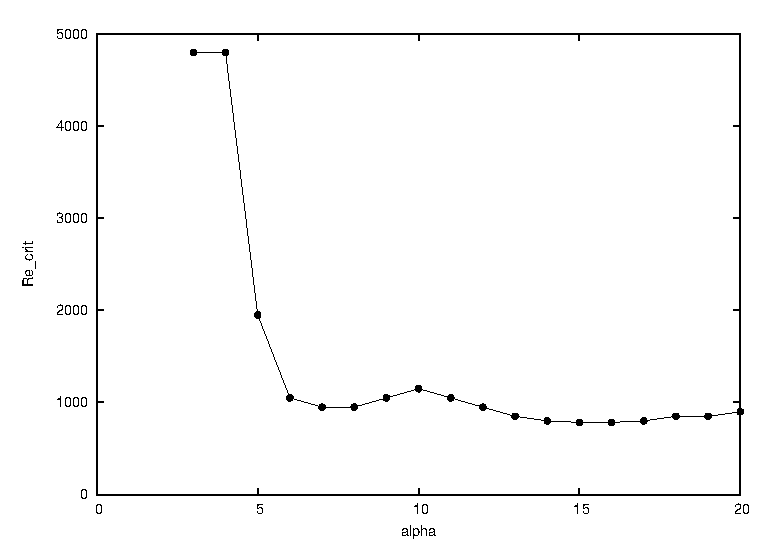
\includegraphics{Re}
\caption{Кривая нейтральной устойчивости}
\label{img:Re_al}
\end{figure}

  \begin{thebibliography}{99}

  \bibitem{method}
  \textit{N.\,Nikitin}, Finite-difference method for incompressible Navier–Stokes equations in 
  arbitrary orthogonal curvilinear coordinates // J. Comput. Phys. 217 (2006) 759–781.

  \bibitem{lin-stability}
  \textit{Etienne Non, Roger Pierre, and Jean-Jacques Gervais}, Linear stability of the 
  three-dimensional lid-driven cavity // Physics of Fluids 18, 084103 (2006)
  
  \bibitem{introduction}
   \textit{Ramanan\.N., Homsy\.G.\.M.} Linear stability of lid-driven cavity flow 
  //Physics of Fluids.~--- 1994.~--- Т. 6.~--- С. 2690.
  
  \bibitem{2DBench}
   \textit{Erturk\.E., Corke\.T.\.C., Gökçöl\.C.} Numerical solutions of 2-D steady incompressible
  driven cavity flow at high Reynolds numbers //International Journal for Numerical Methods in 
  Fluids.~--- 2005.~--- Т. 48.~--- №. 7.~--- С. 747--774.

	\bibitem{KimMoin}
	\textit{J.~Kim and P.~Moin}, Application of a fractional step method to incompressible Navier-Stokes equations//
 J.~Comput.~Phys. 59, 308 (1985).

  \bibitem{betyaev}
   \textit{Бетяев~С.К.} Пролегомены к // РХД, 2006 г. 304 стр
  
  \bibitem{wiki}
   Материал из Википедии~--- свободной энциклопедии [ru.wikipedia.org]

  \bibitem{history}
   История гидродинамики, опубликованно 29-го января 2009 г [http://iproc.ru/interesting/hydro-history]

\end{thebibliography}


\end{document}
